%yright 2007, 2008, 2009 Elsevier Ltd
%% 
%% This file is part of the 'Elsarticle Bundle'.
%% ---------------------------------------------
%% 
%% It may be distributed under the conditions of the LaTeX Project Public
%% License, either version 1.2 of this license or (at your option) any
%% later version.  The latest version of this license is in
%%    http://www.latex-project.org/lppl.txt
%% and version 1.2 or later is part of all distributions of LaTeX
%% version 1999/12/01 or later.
%% 
%% The list of all files belonging to the 'Elsarticle Bundle' is
%% given in the file `manifest.txt'.
%% 

%% Template article for Elsevier's document class `elsarticle'
%% with numbered style bibliographic references
%% SP 2008/03/01

% \documentclass[preprint,11pt]{elsarticle}
\documentclass[final,1p,11pt]{elsarticle}

%\documentclass[final,1p,times]{elsarticle}


%% Use the option review to obtain double line spacing
%%\documentclass[authoryear,preprint,review,12pt]{elsarticle}

%% Use the options 1p,twocolumn; 3p; 3p,twocolumn; 5p; or 5p,twocolumn
%% for a journal layout:
%% \documentclass[final,1p,times]{elsarticle}
%% \documentclass[final,1p,times,twocolumn]{elsarticle}
%% \documentclass[final,3p,times]{elsarticle}
%% \documentclass[final,3p,times,twocolumn]{elsarticle}
%% \documentclass[final,5p,times]{elsarticle}
%% \documentclass[final,5p,times,twocolumn]{elsarticle}

%%% For including figures, graphicx.sty has been loaded in
%% elsarticle.cls. If you prefer to use the old commands
%% please give \usepackage{epsfig}


\usepackage{epsfig}
%\usepackage{cite}
%\usepackage{mcite}
\usepackage{array,tabularx,epsfig,mathrsfs,graphicx,rotating}
\usepackage{ifthen}
\usepackage{amsfonts}
\usepackage{ragged2e}
\PassOptionsToPackage{hyphens}{url}
\usepackage[hyphens]{url}
\usepackage{hyperref}
\usepackage{listings}
\usepackage{lineno}
\usepackage{subfigure}
\usepackage{epstopdf}
% Custom colors
\usepackage{color}
\usepackage{float}
\usepackage{verbatim}
\usepackage{color,soul}
\usepackage{subfigure} 


% to cross text
\usepackage[normalem]{ulem} % either use this (simple) or
\usepackage{soul} % use this (many fancier options)
\usepackage{amsmath,amssymb}

\let\originallesssim\lesssim
\let\originalgtrsim\gtrsim

\DeclareRobustCommand{\lesssim}{%
  \mathrel{\mathpalette\lowersim\originallesssim}%
}
\DeclareRobustCommand{\gtrsim}{%
  \mathrel{\mathpalette\lowersim\originalgtrsim}%
}

\makeatletter
\newcommand{\lowersim}[2]{%
  \sbox\z@{$#1<$}%
  \raisebox{-\dimexpr\height-\ht\z@}{$\m@th#1#2$}%
}
\makeatother


\hypersetup{
  colorlinks=true,
  linkcolor=blue,
  citecolor=blue,
  urlcolor=blue
}




\graphicspath{{figs/}}


\pdfinfo{
   /Author (Chekanov et al)
   /Title  (Studies of granularity of a hadronic calorimeter for tens-of-TeV jets  at a 100 TeV pp collider)
   /CreationDate (D:2017)
   /Subject (PDFLaTeX)
   /Keywords (PDF;LaTeX)
}


\textheight=22cm
\textwidth=14.5cm

\newcommand{\beq}{\begin{equation}}
\newcommand{\eeq}{\end{equation}}
\newcommand{\la}{\langle}
\newcommand{\promc}{{\sc ProMC}}
\newcommand{\ra}{\rangle}
\newcommand{\eps}{\epsilon}
\newcommand{\ud}{\mathrm{d}}
\newcommand{\Ec}{\mathcal{E}}
\newcommand{\Fc}{\mathcal{F}}
\newcommand{\Za}{\mathrm{Z_1}}
\newcommand{\Zb}{\mathrm{Z_2}}
\newcommand{\Zn}{\mathrm{Z_n}}
\newcommand{\F}{\mathrm{F}}

\chardef\til=126
\newcommand{\GEANTfour} {\textsc{geant4}}
\newcommand{\pythia} {\textsc{Pythia8~}}
\newcommand{\pt}{\ensuremath{p_{\mathrm{T}}}}


\journal{}

\begin{document}
%\hfill ANL-HEP-149528
\definecolor{mygreen}{rgb}{0,0.6,0} \definecolor{mygray}{rgb}{0.5,0.5,0.5} \definecolor{mymauve}{rgb}{0.58,0,0.82}

\lstset{ %
 backgroundcolor=\color{white},   % choose the background color; you must add \usepackage{color} or \usepackage{xcolor}
 basicstyle=\footnotesize,        % the size of the fonts that are used for the code
 breakatwhitespace=false,         % sets if automatic breaks should only happen at whitespace
 breaklines=true,                 % sets automatic line breaking
 captionpos=b,                    % sets the caption-position to bottom
 commentstyle=\color{mygreen},    % comment style
 deletekeywords={...},            % if you want to delete keywords from the given language
 escapeinside={\%*}{*)},          % if you want to add LaTeX within your code
 extendedchars=true,              % lets you use non-ASCII characters; for 8-bits encodings only, does not work with UTF-8
 keepspaces=true,                 % keeps spaces in text, useful for keeping indentation of code (possibly needs columns=flexible)
 frame=tb,
 keywordstyle=\color{blue},       % keyword style
 language=Python,                 % the language of the code
 otherkeywords={*,...},            % if you want to add more keywords to the set
 rulecolor=\color{black},         % if not set, the frame-color may be changed on line-breaks within not-black text (e.g. comments (green here))
 showspaces=false,                % show spaces everywhere adding particular underscores; it overrides 'showstringspaces'
 showstringspaces=false,          % underline spaces within strings only
 showtabs=false,                  % show tabs within strings adding particular underscores
 stepnumber=2,                    % the step between two line-numbers. If it's 1, each line will be numbered
 stringstyle=\color{mymauve},     % string literal style
 tabsize=2,                        % sets default tabsize to 2 spaces
 title=\lstname,                   % show the filename of files included with \lstinputlisting; also try caption instead of title
 numberstyle=\footnotesize,
 basicstyle=\small,
 basewidth={0.5em,0.5em}
}


\begin{frontmatter}

\title{
Physics potential of timing layers for future detectors}
%%%%%%%%%%%%%%%%%%%%%%%%%%%%%%%%%%%%%%%%%%%%%%%%%%%%%%%%%%%%%%%

\author[add3]{C.-H. Yeh}
\ead{a9510130375@gmail.com}

\author[add1]{S.V.~Chekanov}
\ead{chekanov@anl.gov}

\author[addDuke]{A.V.~Kotwal}
\ead{ashutosh.kotwal@duke.edu}

\author[add2]{N.V.~Tran}
\ead{ntran@fnal.gov}

\author[add3]{S.-S.~Yu}
\ead{syu@cern.ch}

\address[add3]{
Department of Physics and Center for High Energy and High Field Physics, 
National Central University, Chung-Li, Taoyuan City 32001, Taiwan
}

\address[add1]{
HEP Division, Argonne National Laboratory,
9700 S.~Cass Avenue,
Argonne, IL 60439, USA. 
}

\address[addDuke]{
Department of Physics, Duke University, USA
}

\address[add2]{
Fermi National Accelerator Laboratory
}




\begin{abstract}

\end{abstract}

\begin{keyword}

\end{keyword}
\end{frontmatter}



%%%%%%%%%%%%%%%%%%%%%%%%%%%%%%%%%%%%%%%%%%%%%%%%%%%%%%%%%%%%%%%%%%
\section{Introduction}

Future experiments, such as CLIC \cite{Linssen:1425915}, International Linear Collider (ILC) \cite{Behnke:2013xla}, high-energy LHC (HE-LHC),
future circular $pp$ colliders of the European initiative, FCC-hh~\cite{Benedikt:2206376} and the Chinese initiative, SppC~\cite{Tang:2015qga} will require high precision measurements of particle and jets 
at large transverse momenta. 
The usage of timing information for such experiments  can  provide additional 
information that can be used to improve particle and jet reconstruction, as well as to deal with background events.
For CLIC and FCC, high-precision time stamping will be essential for
background rejection and pile-up mitigation.
For the ILC initiative, timing layers can help dealing with overlap of particle flow objects in high-granular calorimeters.
From physics point of view, timing layers can be used for detection of long-lived particles and identification of Standard Model particles. 
At this moment, conceptional design reports for these future experiments did not fully explore
the benefits of the time of flight (TOF) measurements with tens-of-picosecond resolutions.

In this paper we will explore the benefits of the timing layers for Standard Model (SM) measurements of particles and jets, as well as
investigate the capabilities of timing layers for identification of heavy stable particles which may be produced beyond the Standard Model (BSM).


\section{Proposal}

A generic design of hadronic (electromagnetic) calorimeters for future particle collision experiments (HE-LHC, FCC, CLIC, ILC etc.) 
is based on two main characteristics: (1) high-granularity calorimeters with cells ranged from $3\times 3$ mm$^2$ (for ECAL) to $5\times 5$ cm$^2$  (for HCAL) in sizes.
(2) timing with nanosecond precision that improves background rejection, vertex association, and detection of new particles. 
According to the CPAD report \cite{Ahmed:2019sim}, a development of “picosecond time resolution” for future calorimeters is one of the critical needs. 
Presently. high-granularity calorimeters (with >1 millions channels) with tens of picoseconds resolution represent a 
significant challenge due the large cost.

As a part of the HL-LHC upgrade program, CMS and ATLAS experiments are designing high-precision timing detectors with the time resolution of about 30 ps. 
They are based on silicon sensors that add an extra ``dimension’’ to event reconstruction. 
Such timing capabilities are not fully explored for future detectors beyond the HL-LHC upgrade. 
High-precision timing will be beneficial for new physics searches and b-tagging for all post-LHC experiments. 
For CLIC and FCC, high-precision time stamping will be essential for background rejection and pile-up mitigation. 

Currently, the baseline designs of the high-granularity ECAL and HCAL of the CLIC/FCC detectors have not been 
optimized for precision timing in the range of a few tens of picoseconds. 
The latter is considered as an expensive option for many mullions of channels of these high-granularity detectors. 
This opens an opportunity to investigate a cost-effective “timing layer” (with the time resolution of smaller than 30~ps) for the post-LHC detectors. 
This layer will be installed on front of high-granularity calorimeters, covering both the forward and barrel regions.

In this paper we  will investigate physics advantages for timing layers in the front of calorimeters  
of the post-LHC experiments. 
Typically, thin detectors on front of calorimeters are called ``preshower''. The design goal of such detectors is to count the number of charged
particles in oder to correct for energy loses. The timing information of ``mips'' ( minimum–ionising particles) is not used for particle identifications. 
Unlike the standard pre-shower detector, we propose not only count mips, but also reconstruct high-precision timing and the position.
This timing detector will have a similar granularity as the proposed high-granularity EM calorimeters themselves, 
but will have a sensor technology and readout which is best suited for mip time stamping (not necessarily for energy reconstruction). 
Our proposal is to enclose the EM detectors with two timing layers, one - before the first EM layer, and the second is after the last EM layer (but before
the HCAL). The two layers of the timing detector allows a robust identification of time by correlating the position and timestamps of the particle passing through
the ECAL.

In this paper we will explore this idea using full Monte Carlo simulations. 
A schematic representation of the positions of the timing layers for a generic detector geometry is shown in Fig.~\ref{fig:eff_rad}
In the following, the first timing layer (closest to the interaction point) will be called TL1, while the second timing layer after the electromagnetic calorimeter will be called TL2.

\begin{figure}
\begin{center}
   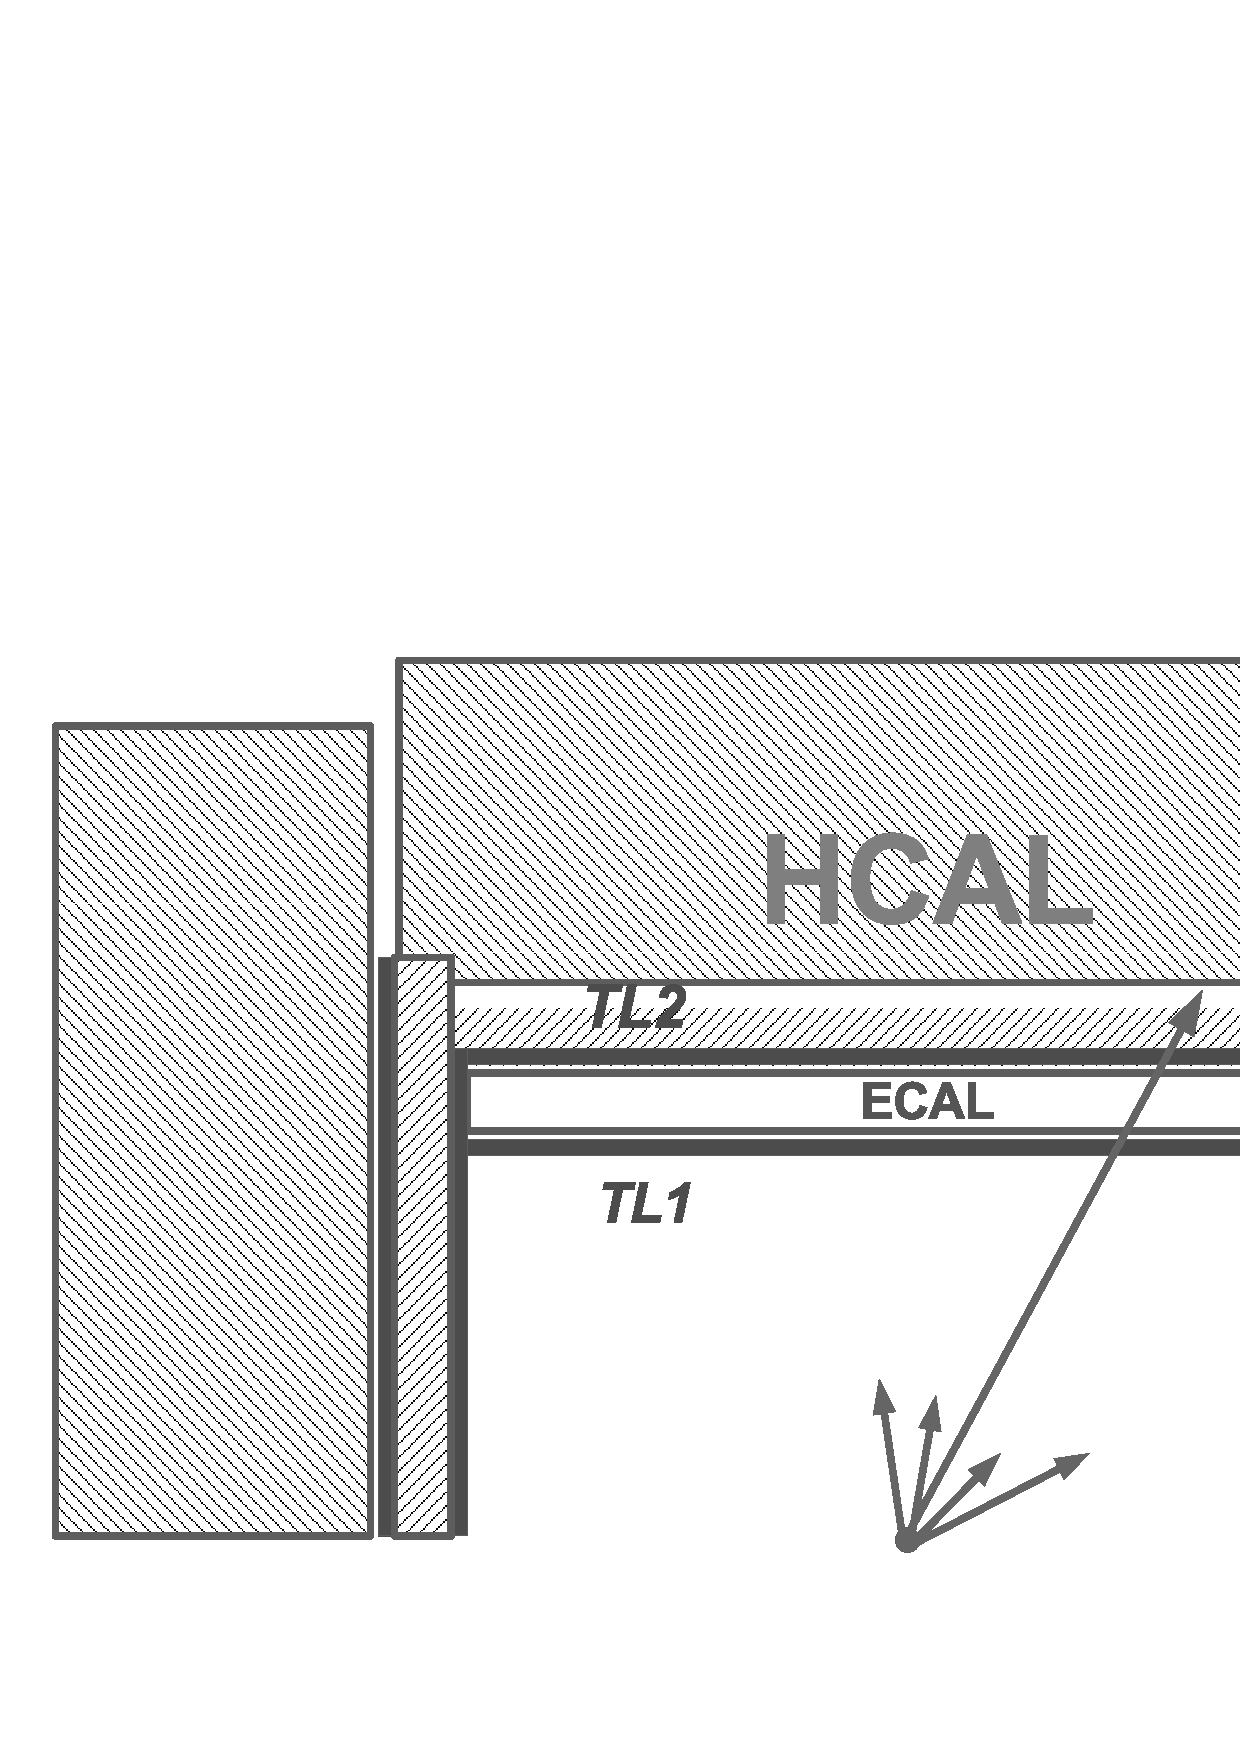
\includegraphics[width=0.8\textwidth]{timing_layer.pdf}\hfill
\end{center}
\caption{An example of positions of the thin timing layers for a generic detector. The thin timing layers  will enclose the electromagnetic calorimeter, allow a reliable reconstruction of the  mip signals with a timing resolution of the order of 10~ps.}
\label{fig:eff_rad}
\end{figure}


There are several reasons why the second timing layer (TL2) can be useful:

\begin{itemize}

\item
It can be used to measure the time of flight between TL2 and TL1, which can be used for identification
of stable massive particles without known production vertex. This is especially important
since the current detectors do not have acceptance for models where the production vertex of the stable heavy particles
is close to the surface of the electromagnetic calorimeter.     
The distance between TL2 and TL1 is typically 0.2-0.4~m (depending on the design of the electromagnetic calorimeter).

This distance is not significant since a particle traveling with the speed of light can travel between TL1 and TL1 within $\sim 1$~ns. 
As we will discuss later, this distance is sufficient for heavy particle identification for a 10-20 ps detector. 


\item
It be useful in cases when a long lived particle (neutral or charged) is produced without precise knowledge of the primary vertex (0,0,0)
due to the beam (or pileup) smearing. 

\item
It allows to correlate the hits with the first layer, and thus provides directionality of the hits. This feature can be useful to
match the hits with the calorimeter cells and to deal with back-scatter 
hits arriving (typically at later time) from the hadronic calorimeter. 

\item
It provides the redundancy for TOF measurements.

\end{itemize}



The second layer of the timing detector can be justified if the recorded time difference for 
hits in the electromagnetic showers is not significantly different from that expected from a particle traveling with the speed of light.
In oder to verify this, we used a full Geant4 (version 10.3)~\cite{Allison2016186} simulation 
of the SiFCC detector \cite{Chekanov:2016ppq} that allows to use the information on hits from the ECAL.
The ECAL is built from a highly segmented silicon-tungsten  with the transverse cell size of $2 \times 2$~cm.
The ECAL has 30 layers built from tungsten pads with silicon readout,
corresponding to 35~X$_{0}$. The first 20 layers use tungsten of 3~mm thickness.
The last ten layers use tungsten layers of
twice the thickness, and thus have half the  sampling fraction.  
The distance between the centers of the last and first ECAL layer is about 240~mm.  

To verify that the time differences between last and first layer of ECAL is close to the time
required for a particle that travels with the speed of light, and can be neglected for the timing layers that
have a timing resolution of the order of 1~ns, a sample of single pions was created with 1 and 10~GeV momenta. 
The particles were reconstructed in the ECAL calorimeter,
and the time difference $\Delta T= T_{\mathrm{last}}-T_{\mathrm{first}}$ of the hits between the last and first ECAL layers was calculated.
Only hits that arrive first were considered.

Figure~\ref{fig:timediff} shows the time distribution for 1 and 10 GeV pions. It can be seen that the peak positions of the distributions are smaller
than 1~ns, as expected for the distance of about 20~cm between  the centers of the last and first layers.
%\footnote{The precision with which the simulations were performed are about 0.2-0.3~ns}. More importantly, the RMS of these distributions are significantly smaller than the 10~ns. 
Therefore, hits will be simultaneous for the
standard 1~ns resolution, i.e. well correlated in time and are identified as a single crossing particle.
If a resolution of the timing layer will be of the order of 10 -- 20~ps, a physics measurement of TOF would be possible.

Figure~\ref{fig:timediff} also shows the hit distribution for (anti)deutrons, denoted as $d^{\pm}$. The distribution are significantly different from $\pi^{\pm}$. On average, 1 GeV
(anti)deutrons should be measured with the time delay of 0.7 -- 1.4~ns between the last and first layers.
The value 0.7 was estimated from the mean position of the Landau distribution used to fit the $d^{\pm}$ curve presented in Figure~\ref{fig:timediff}(a),
while 1.4~ns was obtained for the mean of this distribution. Even for the most conservative 0.7~ns value, there is an indication that 1~GeV
deutrons can be separated from pions that have 0.5~ns time difference. Such a separation can be observed when using a tens-of-picosecond detector.
For 10~GeV particles presented in Figure~\ref{fig:timediff}(b), separation between $d^{\pm}$ and $\pi^{\pm}$ cannot be observed.

In summary, we have illustrated that a typical difference between TL2 and TL1 (which is approximated by the difference
between the last and first layer of the electromagnetic calorimeter) is sufficient for particle identification using the TOF.
As an example, a $d^{\pm}$ can be identified and separated from pions for the momentum less than 1~GeV.
This means that  heavier than deutron particles can also be identified for a momentum larger than 1~GeV.
In the following, we will abstract from the full simulations and calculate the kinematic regions  where identification of heavy stable 
particles is possible.
 

\begin{figure}
\begin{center}
   \subfigure[] { 
   \includegraphics[width=0.45\textwidth]{timeECAL_2layers_1gev1.pdf}\hfill
   }
   \subfigure[] { 
   \includegraphics[width=0.45\textwidth]{timeECAL_2layers_10gev1.pdf}\hfill
   }
\end{center}
\caption{The difference between time of hits between the last and first layer of ECAL for single pions with the transverse momentum 1 and 10 GeV. 
Only first (fastest) hits were considered}
\label{fig:timediff}
\end{figure}



\clearpage 
%%%%%%%%%%%%%%%%%%%%%%%%%%%%%%%%%%%%%%%%%%%%%%%%%%%%%%%%%%%%%%%%%%

%%%%%%%%%%%%%% sections 
\section{Timing layers for single particles}


%\section{Timing layers for ee experiments}

%%%%%%%%%%%%%%% commented out 
\end{comment}


%\section{Timing layers for FCC and jets}

%%%%%%%%%%%%%%% commented out 
\end{comment}


\newpage
%%%%%%%%%%%%%%%%%%%%%% references %%%%%%%%%%%%%%%%%%%%%%%%%%%%%%
%\section*{References}

\bibliographystyle{elsarticle-num}
\def\bibname{\Large\bf References}
%\def\refname{\Large\bf References}
%\pagestyle{plain}
\bibliography{biblio}


\end{document}
